{\bf
%  \subsubsection{Simulations without a radial}
  \section{Artifical radial density bumps with a radially smooth
    viscosity profile}\label{add_sim}
  In \S\ref{density_bump} we found vortices became stronger
  as viscosity is increased, even though linear growth rates
  were reduced. Here, we present additional simulations to clarify the 
  hypothesis that the radially-structured viscosity profile was
  responsible for this result.   

%  For reference we repeated simulation V2 with a floor viscosity
%  $\hat{\nu}_0=10^{-7}$ and all other parameters identical to that in
%  \S\ref{density_bump}. 

  We repeated simulation V2 with the following radially-smooth
  viscosity profile      
  \begin{align}          
    \hat{\nu}\frac{\rho_i       (R,z)}{B(R)} =
    \hat{\nu}_0\left[1+Q(z/H_0) \right]\frac{\rho_i(r_0,z)}{B(r_0)},
  \end{align}                   
  and $Q$ still given by Eq. \ref{step}. (Recall in case V1 the low
  and high viscosity layers occupy $z\in[0,1]H_0$  and
  $z\in[1,2]H_0$ at $R=r_0$, respectively.) We choose a floor viscosity
  of $\hat{\nu}_0=10^{-7}$ to prevent significant viscous diffusion of 
  the initial density bump. This simulation is shown 
  in Fig. , where it is compared to the case employing a
  radially-structured viscosity profile (i.e. the original case V1
  with reduced floor viscosity). 





\begin{figure}
  \centering
  \includegraphics[width=\linewidth]{figures/pdisk_kerz_cases_appendix.ps}
  \caption{{\bf Non-axisymmetric mode amplitude}
    \label{appen}}
\end{figure}

  
}
